% $Id: template.tex 11 2007-04-03 22:25:53Z jpeltier $

\documentclass{vgtc}                          % final (conference style)
%\documentclass[review]{vgtc}                 % review
%\documentclass[widereview]{vgtc}             % wide-spaced review
%\documentclass[preprint]{vgtc}               % preprint
%\documentclass[electronic]{vgtc}             % electronic version

%% Uncomment one of the lines above depending on where your paper is
%% in the conference process. ``review'' and ``widereview'' are for review
%% submission, ``preprint'' is for pre-publication, and the final version
%% doesn't use a specific qualifier. Further, ``electronic'' includes
%% hyperreferences for more convenient online viewing.

%% Please use one of the ``review'' options in combination with the
%% assigned online id (see below) ONLY if your paper uses a double blind
%% review process. Some conferences, like IEEE Vis and InfoVis, have NOT
%% in the past.

%% Figures should be in CMYK or Grey scale format, otherwise, colour
%% shifting may occur during the printing process.

%% These three lines bring in essential packages: ``mathptmx'' for Type 1
%% typefaces, ``graphicx'' for inclusion of EPS figures. and ``times''
%% for proper handling of the times font family.

\usepackage{mathptmx}
\usepackage{graphicx}
\usepackage{times}

%% We encourage the use of mathptmx for consistent usage of times font
%% throughout the proceedings. However, if you encounter conflicts
%% with other math-related packages, you may want to disable it.

%% If you are submitting a paper to a conference for review with a double
%% blind reviewing process, please replace the value ``0'' below with your
%% OnlineID. Otherwise, you may safely leave it at ``0''.
\onlineid{0}

%% declare the category of your paper, only shown in review mode
\vgtccategory{Research}

%% allow for this line if you want the electronic option to work properly
\vgtcinsertpkg

%% In preprint mode you may define your own headline.
%\preprinttext{To appear in an IEEE VGTC sponsored conference.}

%% Paper title.

\title{Laplacian based Dynamic Graph Drawing}

%% This is how authors are specified in the conference style

%% Author and Affiliation (single author).
%%\author{Roy G. Biv\thanks{e-mail: roy.g.biv@aol.com}}
%%\affiliation{\scriptsize Allied Widgets Research}

%% Author and Affiliation (multiple authors with single affiliations).
%%\author{Roy G. Biv\thanks{e-mail: roy.g.biv@aol.com} %
%%\and Ed Grimley\thanks{e-mail:ed.grimley@aol.com} %
%%\and Martha Stewart\thanks{e-mail:martha.stewart@marthastewart.com}}
%%\affiliation{\scriptsize Martha Stewart Enterprises \\ Microsoft Research}

%% Author and Affiliation (multiple authors with multiple affiliations)
\author{Limei Che\thanks{e-mail: chelimei@baidu.com}\\ %
        \scriptsize Baidu, Inc%
\and Xiaoru Yuan\thanks{e-mail:xiaoru.yuan@pku.edu.cn}\\ %
     \scriptsize Peking University%
\and Lun Zhang\thanks{e-mail:zhanglun@baidu.com}\\ %
     \scriptsize Baidu, Inc}

%% A teaser figure can be included as follows, but is not recommended since
%% the space is now taken up by a full width abstract.
%\teaser{
%  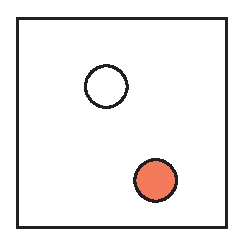
\includegraphics[width=1.5in]{sample.eps}
%  \caption{Lookit! Lookit!}
%}

%% Abstract section.
\abstract{In this paper, we propose a new strategy for drawing dynamic graphs.
We developed an algorithm based on Laplacian constrained distance embedding to 
maintain the topological information of the previous graph layout. It's a online 
algorithm which can preserve user's mental map very well by keeping the dynamic
graph layout consistent stable. Finally, our experimental results suggest this 
new approach to be very effective. 
} % end of abstract

%% ACM Computing Classification System (CCS).
%% See <http://www.acm.org/class/1998/> for details.
%% The ``\CCScat'' command takes four arguments.

\CCScatlist{
 dynamic graph, graph layout algorithm, Laplican matrix, force directed layout,
  stress model
}

%% Copyright space is enabled by default as required by guidelines.
%% It is disabled by the 'review' option or via the following command:
% \nocopyrightspace

%%%%%%%%%%%%%%%%%%%%%%%%%%%%%%%%%%%%%%%%%%%%%%%%%%%%%%%%%%%%%%%%
%%%%%%%%%%%%%%%%%%%%%% START OF THE PAPER %%%%%%%%%%%%%%%%%%%%%%
%%%%%%%%%%%%%%%%%%%%%%%%%%%%%%%%%%%%%%%%%%%%%%%%%%%%%%%%%%%%%%%%%

\begin{document}

%% The ``\maketitle'' command must be the first command after the
%% ``\begin{document}'' command. It prepares and prints the title block.

%% the only exception to this rule is the \firstsection command
%% \firstsection{Introduction}

\maketitle

\section{Introduction}
In many applications,
graphs are widely used to represent social connections, physical networks, or other relationships.
Most of these graphs are changing over time, for example in a social connection, some new people add
in, some old ones leave. To reflect the evolution of the organization or system represented by the graph, 
we can keep a track of snapshots once the graph changed. This kind of sequence graph layout is called
dynamic graph layout problem.

Traditional Graph drawing algorithms are well studied since
early year, layout methods, such as force-directed or stress model layout algorithms are
all concentrate on static graph. They produce a totally new layout each time we run the algorithm. 
Since the dynamic graph sequence is a evolution of a graph, there must be some parts not changed, which
we hope their layout are also not changed. Therefore in dynamic graph drawing, the challenge is that we have to 
layout a current graph aesthetically good while preserving the "mental map" of previous time step.

Mental map was first proposed as a concept in~\cite{Eades:1991:POC}, it means a abstract structural information
a user forms by looking at the layout of a graph. The mental map facilitates memory of a graph or comparison between
it and other graph layouts. Preserving the mental map helps users to quickly recognize the new graph, which
is important in dynamic graph drawing.  



\section{Related Works}

There are algorithms solving the off line dynamic graph drawing, where the whole graph sequence is known in advance.
Early work DynaDag~\cite{North:1996:GD} generated a heuristic method for incremental layout of directed
acyclic graphs drawn as hierarchies.
~\cite{Diehl:2002:GD} proposed a general context preserving algorithm, in which for each graph, it's
layout should have very limited difference between its previous and next time step graph. ~\cite{Kumar:2006:VEC} developed a stratification hierarchical layout algorithm, which not only speed up the general force directed algorithm but also accommodates time-varying graphs.

There are also few works developed online dynamic graph drawing algorithms, where the whole graph sequence is not known ahead. ~\cite{Brandes:1997:GD} introduced random field models for graph layout which based on Bayesian decision theory.

There are some existing algorithms solving the mental map problem,
such as~\cite{Misue:1995:VLC} maintaining the orthogonal ordering, or adding constrains to the graph~\cite{Bhringer:1990:HFC}~\cite{He:1998:C}. 
\section{Laplacian based Dynamic Graph Drawing Algorithm}
In this section we describe our algorithm in detail. 
Given a sequence of online graphs $G_{0}, ..., G_{n}$, where $G_{0} = (V_{0}, E_{0}), ..., G_{n} = (V_{n}, E_{n})$,
the goal of our algorithm is to produce a sequence of layouts $L_{0}, ..., L_{n}$, where $L_{i}$ is a straight line
drawing of $G_{i}$. We first describe how to compute the online dynamic layout $L_{i}, i \ge 1$, when given $L_{i-1}$
and $G_{i}$. Then, we discuss the way to compute initial layout $L_{0}$.

\subsection{Laplacian based dynamic graph layout algorithm}
In the dynamic graph sequence, for each graph $G_{i} = (V_{i}, E_{i})$, each node has a unique id 'UId'.
Through this unique id, we can recognize the same nodes in different time step.
The following are the basic steps of our algorithm:
\begin{enumerate}
    \item Calculate initial node positions from previous graph layout $L_{i-1}$.
    \item Run force-directed layout algorithm.
    \item Run Laplacian Constrained Distance Embedding algorithm to refine the mental map.
\end{enumerate}

\textbf{Step 1:} For each node $v$ in $G_{i}$, which is existed in $G_{i-1}$, copy
the coordinates from $L_{i-1}$ to this node; for those new added nodes, calculate their coordinates
according to their neighbors as follows: if node $v$ has more than one positioned neighbors, then 
this node is assigned the barycenter of all its positioned neighbours; if node $v$ has only one positioned
neighbour $p$, select a random position on the circle which take $p$ as center of this circle, and the average edge length 'avg_edge_length' of $L_{i-1}$ as radius; if node $v$ has no positioned neighbour, then it can be placed
randomly.

\textbf{Step 2:} Run force-directed layout algorithm starting from the positions assigned in step 1. Here we use 
the simulated annealing force-directed layout algorithm~\cite{Davidson:1996:ATG} to adjust the layout $L_{i}$. For
different nodes we set different cooling parameters. In order to keep the existed nodes as stable as possible, we
have to frozen these nodes which copy coordinates from $L_{i-1}$, only small movements allowed. For those nodes that
are totally random positioned, we should let them move far away enough to find their best positions, so the cooling 
parameter should be high. In our implementation, scores of 0.25, 0.5, 0.75 and 1 are assigned to nodes positioned
copied from $L_{i-1}$, at the barycenter of two or more neighbors, according to one neighbor, and totally random ones,
respectively. 

\textbf{Step 3:} Although we have preserved user mental map by setting a small parameter of cooling step, but it's still far from stable. The nodes both existed in graph $G_{i-1}$ and $G_{i}$ move a lot by the forces from 
new added and disappeared nodes and edges. Inspired by the Laplacian constrained graph layout algorithm~\cite{Yuan:2012:TVCG}, we can take the subgraph consist of nodes that are copied from $L_{i-1}$ as
a user input subgraph, then run the Laplacian constrained distance embedding algorithm. 

\subsection{Initial layout of dynamic graph}


\section{Experiment}
\section{Conclusion}

\section{Exposition}


Lorem ipsum dolor sit amet, consetetur sadipscing elitr, sed diam
nonumy eirmod tempor invidunt ut labore et dolore magna aliquyam erat,
sed diam voluptua. At vero eos et accusam et justo duo dolores et ea
rebum. Stet clita kasd gubergren, no sea takimata sanctus est Lorem
ipsum dolor sit amet. Lorem ipsum dolor sit amet, consetetur
sadipscing elitr, sed diam nonumy eirmod tempor invidunt ut labore et
dolore magna aliquyam erat, sed diam voluptua.

\begin{equation}
 \sum_{j=1}^{z} j = \frac{z(z+1)}{2}
\end{equation}

Lorem ipsum dolor sit amet, consetetur sadipscing elitr, sed diam
nonumy eirmod tempor invidunt ut labore et dolore magna aliquyam erat,
sed diam voluptua. At vero eos et accusam et justo duo dolores et ea
rebum. Stet clita kasd gubergren, no sea takimata sanctus est Lorem


rebum. Stet clita kasd gubergren, no sea takimata sanctus est Lorem
ipsum dolor sit amet.

\begin{table}
  \caption{Vis Paper Acceptance Rate}
  \label{vis_accept}
  \scriptsize
  \begin{center}
    \begin{tabular}{cccc}
      Year & Submitted & Accepted & Accepted (\%)\\
    \hline
      1994 &  91 & 41 & 45.1\\
      1995 & 102 & 41 & 40.2\\
      1996 & 101 & 43 & 42.6\\
      1997 & 117 & 44 & 37.6\\
      1998 & 118 & 50 & 42.4\\
      1999 & 129 & 47 & 36.4\\
      2000 & 151 & 52 & 34.4\\
      2001 & 152 & 51 & 33.6\\
      2002 & 172 & 58 & 33.7\\
      2003 & 192 & 63 & 32.8\\
      2004 & 167 & 46 & 27.6\\
      2005 & 268 & 88 & 32.8\\
      2006 & 228 & 63 & 27.6
    \end{tabular}
  \end{center}
\end{table}

\begin{figure}[htb]
  \centering
  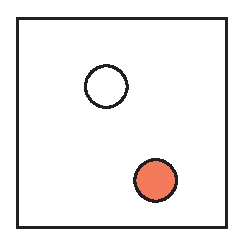
\includegraphics[width=1.5in]{sample.eps}
  \caption{Sample illustration.}
\end{figure}

\subsection{Mezcal Head}

Duis autem~\cite{Lorensen:1987:MCA} vel eum iriure dolor in hendrerit
in vulputate velit esse molestie consequat, vel illum dolore eu
feugiat nulla facilisis at vero eros et accumsan et iusto odio
dignissim qui blandit praesent luptatum zzril delenit augue duis
dolore te feugait nulla facilisi. Lorem ipsum dolor sit amet,
consectetuer adipiscing elit, sed diam nonummy nibh euismod tincidunt
ut laoreet dolore magna aliquam erat volutpat%
\footnote{Footnotes appear at the bottom of the column}.


\subsubsection{Ejector Seat Reservation}

Ut wisi enim ad minim veniam, quis nostrud exerci tation ullamcorper
suscipit lobortis nisl ut aliquip ex ea commodo
consequat~\cite{Nielson:1991:TAD}. Duis autem vel eum iriure dolor in
hendrerit in vulputate velit esse molestie consequat, vel illum dolore
eu feugiat nulla facilisis at vero eros et accumsan et iusto odio
dignissim qui blandit praesent luptatum zzril delenit augue duis
dolore te feugait nulla facilisi.


\paragraph{Rejected Ejector Seat Reservation}

Ut wisi enim ad minim veniam, quis nostrud exerci tation ullamcorper
suscipit lobortis nisl ut aliquip ex ea commodo consequat. Duis autem
vel eum iriure dolor in hendrerit in vulputate velit esse molestie

\section{Conclusion}

Lorem ipsum dolor sit amet, consetetur sadipscing elitr, sed diam
nonumy eirmod tempor invidunt ut labore et dolore magna aliquyam erat,
sed diam voluptua. At vero eos et accusam et justo duo dolores et ea
rebum. Stet clita kasd gubergren, no sea takimata sanctus est Lorem
ipsum dolor sit amet. Lorem ipsum dolor sit amet, consetetur
sadipscing elitr, sed diam nonumy eirmod tempor invidunt ut labore et
dolore magna aliquyam erat, sed diam voluptua. At vero eos et accusam
et justo duo dolores et ea rebum. Stet clita kasd gubergren, no sea
takimata sanctus est Lorem ipsum dolor sit amet. Lorem ipsum dolor sit
amet, consetetur sadipscing elitr, sed diam nonumy eirmod tempor
invidunt ut labore et dolore magna aliquyam erat, sed diam
voluptua. At vero eos et accusam et justo duo dolores et ea
rebum. Stet clita kasd gubergren, no sea takimata sanctus est Lorem
ipsum dolor sit amet.

Lorem ipsum dolor sit amet, consetetur sadipscing elitr, sed diam
nonumy eirmod tempor invidunt ut labore et dolore magna aliquyam erat,
sed diam voluptua. At vero eos et accusam et justo duo dolores et ea
rebum. Stet clita kasd gubergren, no sea takimata sanctus est Lorem
ipsum dolor sit amet. Lorem ipsum dolor sit amet, consetetur
sadipscing elitr, sed diam nonumy eirmod tempor invidunt ut labore et
dolore magna aliquyam erat, sed diam voluptua. At vero eos et accusam
et justo duo dolores et ea rebum.

%% if specified like this the section will be ommitted in review mode
\acknowledgements{
The authors wish to thank A, B, C. This work was supported in part by
a grant from XYZ.}

\bibliographystyle{abbrv}
%%use following if all content of bibtex file should be shown
\nocite{*}
\bibliography{reference}
\end{document}
